
\begin{savequote}[15cm]
  \raggedleft
  \sffamily
  Tables, tables, where do I put my tables?
  \qauthor{Anonymous}
\end{savequote}
\chapter{Tables, tables}

Although \LaTeX has its strengths, it is not particularly time effecient when you want to design nice tables.

A spreadsheet (excel, libreoffice calc) may serve you better than having to hand craft tables.

To show what handcrafting can mean you might want to take a look at the sources of the next table.

{
    \setlength{\TabColumnWidth}{24mm}
    \footnotesize\sffamily
    
    \begin{longtable}{| g{.8\TabColumnWidth} | g{\TabColumnWidth} | g{\TabColumnWidth}| g{\TabColumnWidth}| g{\TabColumnWidth}| g{\TabColumnWidth}|}
        \caption{Research results summarized} \label{tab:results}\\
        \hline \rowcolor{Gray}
        \headcell{Criteria} & \headcell{Alt 1} & \headcell{Alt 2} & \headcell{Alt 3} & \headcell{Alt 3} \\\hline
        \endfirsthead
        
        \rowcolor{Gray}
        \multicolumn{5}{l}{{\bfseries \tablename\ \thetable{} Research results summarized -- continued from previous page}} \\\hline
        
        \rowcolor{Gray}
        \headcell{Criteria} & \headcell{Alt 1} & \headcell{Alt 2} &\headcell{Alt 3} & \headcell{Alt 4} \\ \hline
        \endhead
        
        \hline \rowcolor{Gray}\multicolumn{5}{|r|}{{Continued on next page}}\\ \hline
        \endfoot
        
        \hline \hline
        \endlastfoot
        
        % ------ Table content start ------
        \firstcell{.NET 6.0\\Support} & 
        \itemcell{
            \itemC Yes
        } &
        \itemcell{
            \itemC Yes
        } & 
        \itemcell{
            \itemC Yes
            \itemW Since 2022-08-25
        } &
        \itemcell{
            \itemC Yes
        }\\\hline

        
        \firstcell{Documentation} &
        % Traeger
        \itemcell{
            \itemC Online Documentation
            \itemC Examples
        } &
        % softing
        \itemcell{
            \itemC CHM Documentation
            \itemC Examples
            \itemC YouTube Tutorials
        } &
        % UA
        \itemcell{
            \itemC Code Documentation
            \itemC Examples
            \itemC Tutorials
        } &
        % OPC
        \itemcell{
            \itemC GitHub Documentation
        }
        \\\hline

        
        \firstcell{Security} &
        % Traeger
        \itemcell{
            \itemC Signed
            \itemC Sign  \& Encrypt
            \itemC Certificates
        } &
        % softing
        \itemcell{
            \itemC Signed
            \itemC Sign \& Encrypt
            \itemC Certificates
        } &
        % UA
        \itemcell{
            \itemC Signed
            \itemC Sign \& Encrypt
            \itemC Certificates
        } &
        % OPC
        \itemcell{
            \itemC Signed
            \itemC Sign \& Encrypt
            \itemC Certificates
        } \\\hline

        
        \firstcell{License types} &
        % Traeger
        \itemcell{
            \itemC Single Developer License
            \itemC Branch License (=postal address)
        } &
        % softing
        \itemcell{
            \itemC Single Developer License
            \itemX Branch License
        } &
        % UA
        \itemcell{
            \itemC Single Developer License
            \itemX Branch License
        } &
        % OPC
        \itemcell{
            \itemC Branch License
        } \\\hline

        
        \firstcell{Support} &
        % Traeger
        \itemcell{
            \itemC inc. 12 months  Top Level Support
            \itemC Support and  update renewal 12  months (price  depending on  license)
        } &
        % softing
        \itemcell{
            \itemC Dedicated  support team
            \itemW Support is valid  for 3 years and can be extended in 1-year steps afterward
        } &
        % UA
        \itemcell{
            \itemC Includes first-year maintenance  package
            \itemW Includes only  15 support  incidents
        } &
        % OPC
        \itemcell{
            \itemC No support  nor guarantees
        } \\\hline

        
        \firstcell{License} &
        % Traeger
        \itemcell{
            \itemC Unlimited  license lifetime
            \itemC No royalty fees
        } &
        % softing
        \itemcell{
            \itemC All Software  updates included
            \itemC Unlimited runtime  of the \acrshort{sdk} past  of maintenance  contract
            \itemC No royalty fees
            \itemC Available in  source code and  binary
        } &
        % UA
        \itemcell{
            \itemC Includes one  UaModeler license
            \itemC Includes one  UaExpert license
        } &
        % OPC
        \itemcell{
            \itemC OPC Foundation  license
            \itemC Open source
        } \\\hline

        
        \firstcell{Price\\}\footnote{\label{footnote:vat}VAT excluded} &
        % Traeger
        \itemcell{
            \itemC Single developer  license\\Client: \hfill{}990€\\Server: \hfill{}2.175€\\Combined:\hfill{}2.600€
            \itemC Branch license\\Client: \hfill{}2.000€\\Server: \hfill{}4.350€\\Combined:\hfill{}5.200€
        } &
        % softing
        \itemcell{
            \itemC Single developer  license\\Client: \hfill{}3.150€\\Server: \hfill{}6.150€\\Combined:\hfill{}9.662€
        } &
        % UA
        \itemcell{
            \itemC Single seat  developer license\\Combined:\\\hfill{}4.900€
            \itemW Further support costs yearly:\\\hfill{}1.470€
        } &
        % OPC
        \itemcell{
            \itemC Free
        } \\\hline

        
        \firstcell{Costs for 5 yrs} \cref{footnote:vat}\footnote{with no prior license} &
        % Traeger
        \itemcell{
            \itemC 8.320€
            \itemC Unlimited  developers
        } &
        % softing
        \itemcell{
            \itemC 15.862€
            \itemC One developer
        } &
        % UA
        \itemcell{
            \itemW 10.780€
            \itemC One developer
        } &
        % OPC
        \itemcell{
            \itemC 0€
            \itemC Unlimited  developers
        } \\\hline

        
        \firstcell{Other} &
        % Traeger
        \itemcell{
            \itemC Branch license  (Client \& Server)  already bought
            \itemW Further support  costs yearly 780€
        } &
        % softing
        \itemcell{
            \itemC Integrated log  system
        } &
        % UA
        \itemcell{
            \itemW May not be stable  on .NET 6.0
        } &
        % OPC
        \itemcell{
            \itemC Limited features
        } \\\hline

        
        \firstcell{Weblink} &
        % Traeger
        \itemcell{
            \itemU \href{https://www.fontys.nl}{Fontys Home}
        } &
        % softing
        \itemcell{
            \itemU \href{https://github.com/homberghp/bachelor_thesis_tips}{This document}
        } &
        % UA
        \itemcell{
            \itemU \href{https://www.unified-automation.com/products/server-sdk/net-ua-server-sdk.html}{UA~Bundle}
        } &
        % OPC
        \itemcell{
            \itemU \href{https://github.com/OPCFoundation/UA-.NETStandard}{OPC~Foundation General}
        }\\
    \end{longtable}
}


\section{The easy way or the high way}

Luckily, spreadsheets can also create good looking tables. That is their bread and butter right?
And of course, what applies to diagrams and codelistings applies here too. We want to be able to zoom in to any depth
of our liking without landing in the world of MineCraft, so export from the spreadsheet using svg(and convert to pdf) or pdf directly. That way you can have the reviewer zoom in and select text to make his/her remarks.

Here are some examples.

\begin{table}
  \caption{We commonly put table captions at the top}
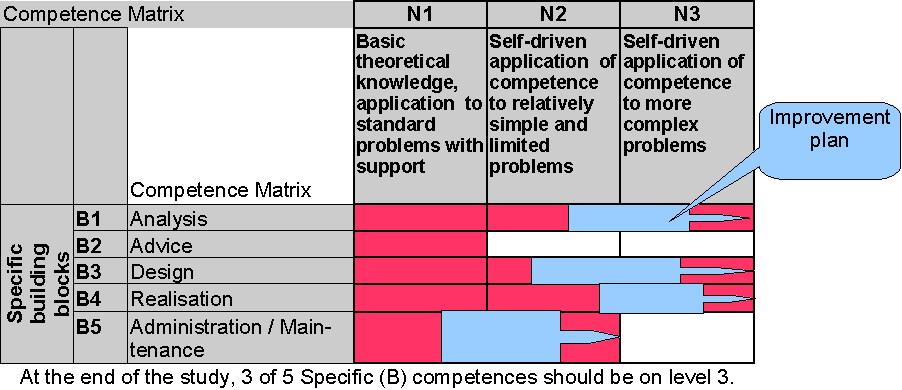
\includegraphics{tables/matrixExample-crop.pdf}   
\end{table}

Note that the \textit{enviroment} is table, but we include the table as if it were an image with includegraphics.

\begin{table}
  \caption{Another table, this time made with word, but included as pdf!}
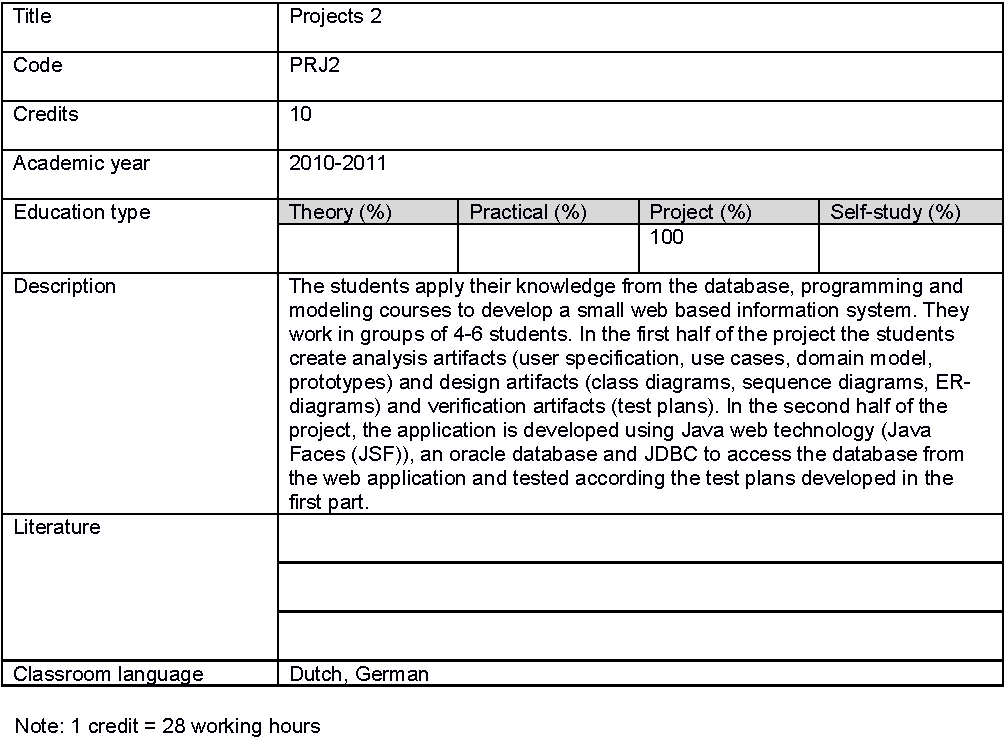
\includegraphics{tables/md_prj2-crop.pdf}   
\end{table}

\begin{table}
  \caption{ESD, still going strong?}
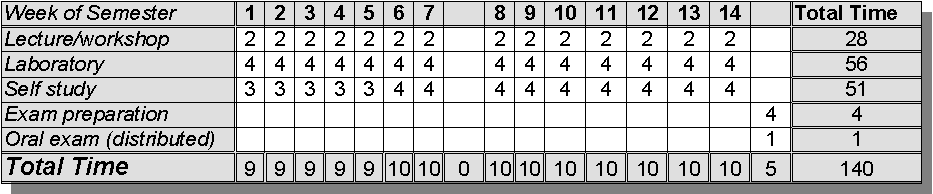
\includegraphics{tables/timetable-crop.pdf}
\end{table}


To preparev the tables, export or print \textit{a selection} of the spreadsheet to pdf without header and footer.
Then use pdfcrop, part of TeXLive, to crop the pdf to just the content. With cropping you remove the white space around the table, so it becomes its true size and appearance.

You can embellish the table in the spreadsheet as much as you like. The fruit of that work will then be visible in is appearance in you report.

